\chapter{Background}\
\label{chap:background}
This section tackles the fundamental principles and groundwork of the theory encompassing concepts, terminology, and methodologies related to search engines as applied within this thesis. Section \ref{sec:web-search-engine} dives into the essential components and characteristics required to implement the search engine discussed in this thesis. Section \ref{sec:crawler} provides a comprehensive examination of the crawler's specifications and architecture. Section \ref{sec:indexing} offers an in-depth explanation of the fundamental indexing terms and concepts essential to this thesis, while Section \ref{sec:ranking} explores the ranking score used in this research.


\section{Web Search Engine}
\label{sec:web-search-engine}
Web Search Engine is software that collects information from the web and indexes them efficiently to optimize the searching process by the end user. When users enter their queries to ask for information, the engine performs queries, looks up the pre-built organized index, and returns relevant results. Search Engine Results Pages, known as SERPs, present the returned results. The result is then ranked based on predefined criteria. 

Web search engines use web crawlers or spiders to collect and harvest the internet, jumping from one page to another. Each page can contain several links. The crawler's task is to find the links, visit them, and harvest them. Followed by crawlers, indexing is the next process where information is organized and optimized for search.

\begin{figure}[h]	
     \centering
         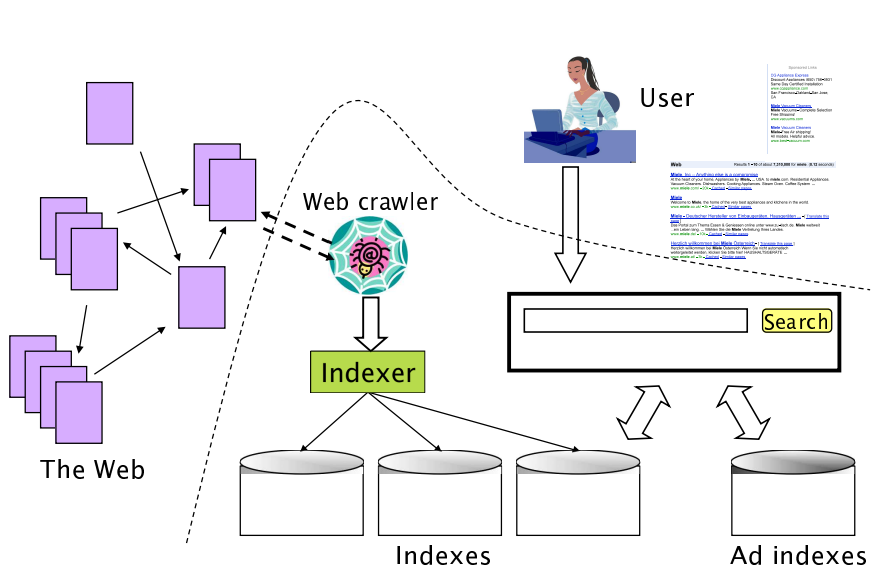
\includegraphics[width=10cm]{images/engine_components.png}
              \caption{An overview of a generic search engine system.}
     \label{fig:search-engine-overvoew}
\end{figure}

\subsection{Requierments and Features}
Regardless of their implementation and design, all search engines share certain features and prerequisites crucial for their effectiveness. Below is a compilation of the most essential features: 

\begin{itemize}
	\item[] \textbf{Web Crawling and Indexing:} As shown in Figure \ref{fig:search-engine-overvoew}, the initial step in the search engine's operation is web crawling. Crawlers initiate the process by connecting to the web and downloading the required pages. Subsequently, indexing comes into play, where the downloaded files are organized and indexed to enhance querying and search efficiency. Parsing the downloaded pages can be carried out in either the crawling phase or during indexing, and Scriburg, this parsing occurs during the crawling process. It is worth noting that, in Scriburg, pages are not downloaded; the targeted documents are parsed, stored in the database, and the pages themselves are discarded.
  \item[] \textbf{Ranking and Relevancy:} As indicated in Figure \ref{fig:search-engine-overview}, when users input a query to search for relevant documents, they face the Search Engine Results Pages (SERP). Users typically focus on the top results while overlooking the lower results. Hence, we must maintain relevancy. Ensuring relevance is a challenging task. Ranking the discovered documents and prioritizing the most pertinent documents at the top and the less relevant ones further down is crucial. 
  \item[] \textbf{Scalability and Performance:} A distributed system is essential for managing the extensive data and traffic demands. A load balancer is critical in distributing the crawling tasks efficiently among nodes and threads. In this, we will discuss the implemented loading balance mechanism to distribute the crawling tasks among the crawlers. 

\end{itemize}

\section{Cralwer}
\label{sec:crawler}
Web crawler or spider is a software which gathers pages information from the web, to prived the necessary data to the Indexer to build a search engine. The essential role of crawlers is to effectively and reliably collect as much information from the web as possible. This thesis invests more time on this component than the Indexer as it serves as the bottleneck to the Search engine performance. There are different types and categories of crawlers. The first category is  \textbf{Universal or Broad crawler}. This category of web crawlers does not confine itself to webpages of a specific topic or domain; instead, they continuously traverse links without limitations, collecting all encountered webpages. Google and Bing use this type of crawler. The second category is called \textbf{Preferential crawler (Focused crawler)}. Focused crawlers target specific topics, themes, or domains \cite{wires}. They are designed to gather information from a particular domain or subject area, providing specialized search results. In this thesis, a Focused crawler has been implemented and used. 

\subsection{Cralwer Specifications}
\label{sec:cralwer-specifications}
Crawlers can display a diverse range of features and specifications. Nevertheless, certain essential elements must be incorporated, while others are critical for ensuring a reliable and functional crawler. Further details can be explored in the book referenced as \cite{introduction-ir}.

\begin{itemize}
\item[] \textbf{Robustness:} Web crawlers can be fragile and easy to break due to the nature of the dynamic contents on the web and the internet connection. Crawlers may encounter broken links, leading to errors and incomplete indexing. Some websites may block or ban crawlers' IP addresses if they perceive them as causing too much traffic or disruption. Web crawlers must identify those edge cases and obstacles and tackle them.

\item[] \textbf{Politeness:} The crawler implementation can be unintentionally dangerous if incorrectly designed. A Denial of service DoS and a Distributed Denial of service DDoS attacks can occur due to an irresponsible crawler implementation. Hence, crawlers must respect website policies and avoid breaking up web services and loading the servers.

\item[] \textbf{Performance and Efficiency:} The crawling system should use various resources, such as processing power, storage capacity, and network bandwidth. Moreover, the crawler should be able to function in distributed microservices across multiple machines.

\item[] \textbf{Freshness:} Obtaining recent versions of previously accessed pages, ensuring the search index remains updated.
\end{itemize}

\subsection{Crawler Architecture}

The simple crawler architecture includes the following fundamental modules, as shown in the following Figure \ref{fig:web-crawler-arch
}. The Fetch module communicates with the internet and collects the pages passed by the URL Frontier module using HTTP requests from the URLs. The URL frontier module contains a list of the URLs that need to be fetched by the Fetch module. Parsing module that takes the page content found by the Fetch module and parses the page content to find the next links to be passed to the URL frontier and also to parse any value needed from the page, like text and images. The following step involves screening the parsed document to eliminate previously visited URLs, duplicate content, and pages that are prohibited by the website. The Domain Name System (DNS)\footnote{The Domain Name System (DNS) is a distributed naming system for internet resources, linking information to domain names.} resolution module identifies the web server from which to retrieve the page indicated by a given URL \cite{introduction-ir}. The DNS will be excluded in this thesis and will not be discussed. 

\begin{figure}[h]	
     \centering
     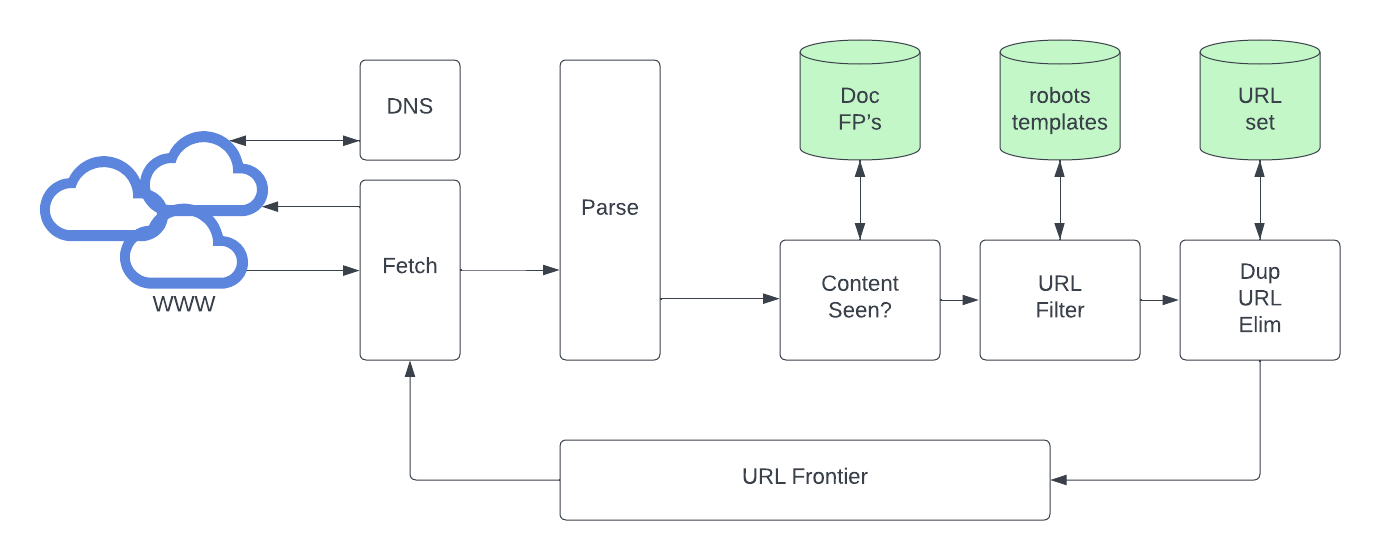
\includegraphics[width=10cm]{images/crawler_architecture.png}
     \caption{A generic web crawler architecture overview \cite{introduction-ir}.}
     \label{fig:web-crawler-arch}
\end{figure}

The crawling process begins with adding a seed URL to the URL frontier as a starting point. The crawler retrieves and stores the corresponding page for parsing. The page's textual content, embedded links, and images are extracted during parsing, with the content prepared for use by the search engine's indexer. Each parsed link undergoes filtering to determine if it is eligible for inclusion in the URL frontier.

Following parsing, a filtering process is essential. Firstly, the content's uniqueness is verified using a fingerprint, often a checksum stored in Doc FP's database. Next, newly parsed URLs are filtered based on various criteria, such as excluding URLs outside the target country or restricted URLs. Domain administrators can specify additional filtering rules, often outlined in a Robots.txt\footnote{More information about Robots.txt can be found in the following link:  \url{https://en.wikipedia.org/wiki/Robots.txt}} file. The Robots Exclusion Protocol (Robots.txt) file is a widely recognized standard websites use to communicate which parts of the site are accessible to web crawlers and other web robots.

The Robots.txt file can be obtained at the start of the crawling process and cached for efficiency, assuming it will not change during crawling. This approach is more efficient than making repeated HTTP requests for the file, reducing the number of requests and server load. Including Robots.txt in the crawling process aligns with the politeness guidelines discussed in the crawler specifications section \ref{sec:cralwer-specifications}.

\subsection{Crawler Data Structure}
Scriburg employs two distinct data structures for its crawling implementation: it utilizes Breadth First Search (BFS) and Depth First Search (DFS).

\textbf{Breadth First Search (BFS):} Considering the link planned for crawling as a vertex, it is worth noting that web pages can be conceptualized as graphs rather than trees. In contrast to trees, graphs can include cycles, which means we might revisit the same vertex. For instance, a basic illustration of this is the home page link, which essentially represents a self-loop in a graph. We can maintain two distinct data structures to prevent processing a vertex multiple times: "Visited" and "Not Visited" vertices. The "Visited" vertices can be stored in a hashmap where the link serves as the key, and the boolean value represents whether the link has already been visited (true for visited, false for unvisited). The second data structure is a queue containing links that still need to be visited.

\begin{figure}[ht] 
  \begin{subfigure}[b]{0.5\textwidth}
    \centering
    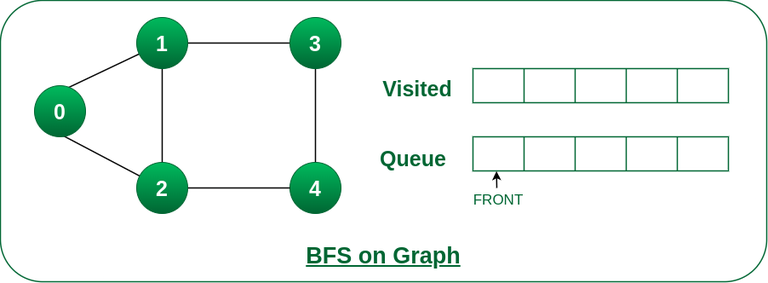
\includegraphics[width=0.75\textwidth]{images/bfs-1.png} 
    \caption{Initial condition} 
    \label{fig7:a} 
    \vspace{4ex}
  \end{subfigure}%% 
  \begin{subfigure}[b]{0.5\textwidth}
    \centering
    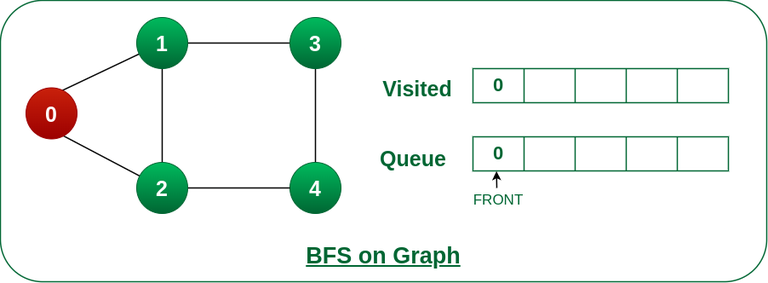
\includegraphics[width=0.75\textwidth]{images/bfs-2.png} 
    \caption{Visit the 0 vertex}  
    \label{fig7:b} 
    \vspace{4ex}
  \end{subfigure} 
  \begin{subfigure}[b]{0.5\textwidth}
    \centering
    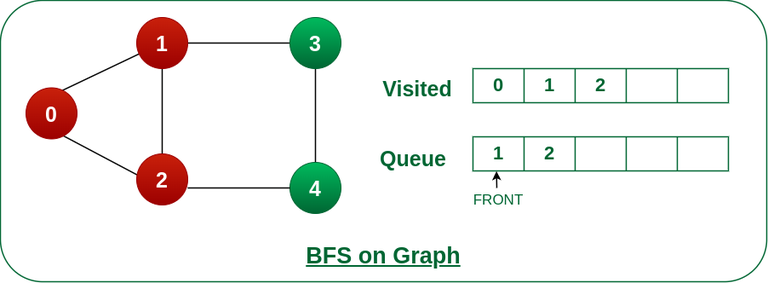
\includegraphics[width=0.75\textwidth]{images/bfs-3.png} 
    \caption{Visit 1 and 2 vertices} 
    \label{fig7:c} 
  \end{subfigure}%%
  \begin{subfigure}[b]{0.5\textwidth}
    \centering
    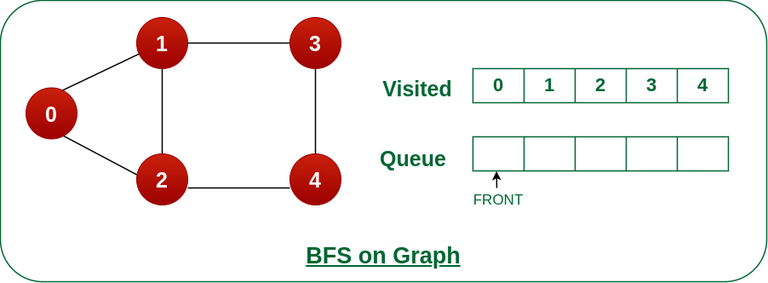
\includegraphics[width=0.75\textwidth]{images/bfs-4.png} 
    \caption{Completed condition} 
    \label{fig7:d} 
  \end{subfigure} 
  \caption{Illustration of the Breadth First Search or BFS for a Graph algorithm.
 \cite{bfs}}
  \label{fig:bfs} 
\end{figure}

The traversal proceeds from the root by visiting all the nodes within a specific level before moving on to the next level. This is accomplished by employing a queue. The unvisited nodes adjacent to the current level are enqueued, while the nodes in the current level are marked as visited and dequeued. One way to perceive this is by initiating the crawling process from the seed URL page, which serves as the root node, and the next level represents all the links discovered within the root page.

Figure \ref{fig:bfs} illustrates the BFS algorithm in operation to enhance visual understanding. Let us visualize a seed URL, denoted as vertex 0. The seed URL page contains two additional links, 1 and 2. The page represented by vertex 1 contains three links: 0, 2, and 3. Similarly, the page associated with vertex 2 includes three links: 0, 1, and 4. Our primary aim is to visit all nodes (links), which is the fundamental objective of the crawler. The crawler must avoid infinite looping and avoid revisiting previously visited nodes (links).

Initially, the queue and the visited hashmap are empty of any entries, which is the ideal state of the crawler. As the crawler launches on its crawling journey, it begins by pushing the seed URL, identified as node 0, into the queue and setting it as visited after visiting it. Subsequently, once the 0 page has been visited, it is dequeued, and the following two discovered links, 1 and 2, are added to the queue. These links, 1 and 2, are similarly dequeued and recorded in the hashmap as visited links. This process persists until the queue is empty, ensuring all the links (nodes) have been visited. It is essential to observe that when the crawler encounters a loop or a link pointing to a previously visited link, we can verify if the link has been marked as visited in the hashmap before introducing it to the queue.

In the case of a random graph, the time complexity of BFS is denoted as $O(|V|+|E|)$ where $|V|$ is the number of vertices and $|E|$ is the number of edges in the graph \cite{introduction-to-algorithms}. This time complexity depends on the graph's topology, where $O(|E|)$ can range from $O(|V|)$ (in the scenario of an acyclic graph) to $O(|V|^2)$ (if all vertices are interconnected). Consequently, the time complexity fluctuates between $O(|V| + |V|) = O(|V|)$ and $O(|V| + |V|^2) = O(|V|^2)$, depending on the specific topology of your graph. The graph assumes an acyclic structure in the existing crawler implementation since it prevents revisiting previously visited links. Consequently, the time complexity for the crawler is $O(|V|)$.
\begin{figure}[ht] 
  \begin{subfigure}[b]{0.5\textwidth}
    \centering
    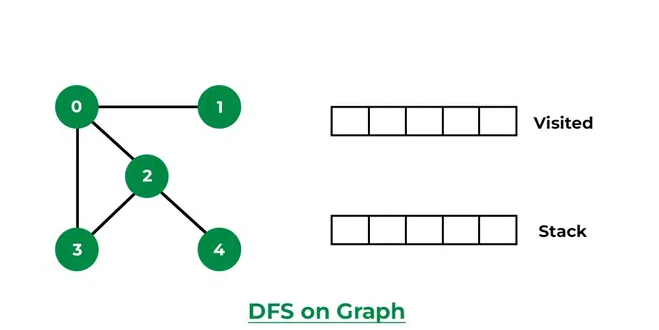
\includegraphics[width=0.75\textwidth]{images/dfs-1.png} 
    \caption{Initial condition} 
    \label{fig7:a} 
    \vspace{4ex}
  \end{subfigure}%% 
  \begin{subfigure}[b]{0.5\textwidth}
    \centering
    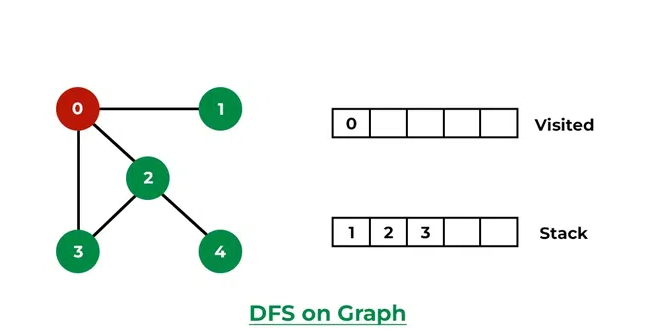
\includegraphics[width=0.75\textwidth]{images/dfs-2.png} 
    \caption{Visit the 0 vertex}  
    \label{fig7:b} 
    \vspace{4ex}
  \end{subfigure} 
  \begin{subfigure}[b]{0.5\textwidth}
    \centering
    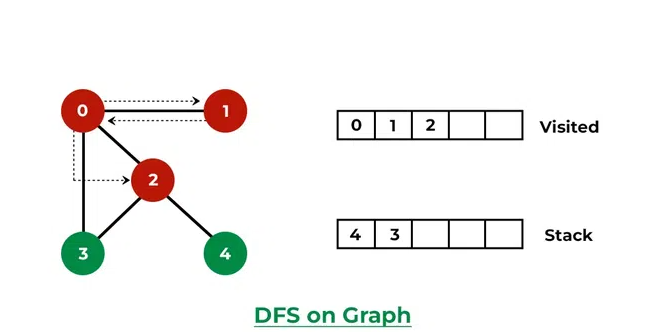
\includegraphics[width=0.75\textwidth]{images/dfs-3.png} 
    \caption{Visit 1 and 2 vertices} 
    \label{fig7:c} 
  \end{subfigure}%%
  \begin{subfigure}[b]{0.5\textwidth}
    \centering
    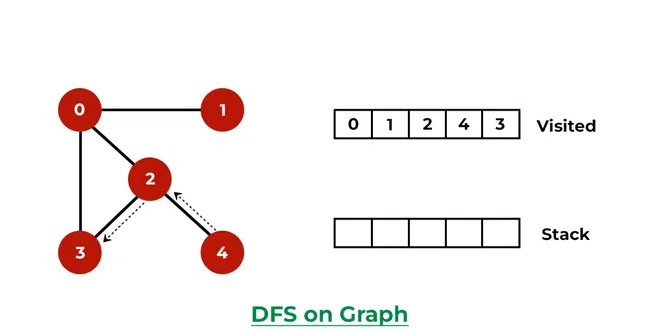
\includegraphics[width=0.75\textwidth]{images/dfs-4.png} 
    \caption{Completed condition} 
    \label{fig7:d} 
  \end{subfigure} 
  \caption{Illustration of various images}
  \label{fig:dfs} 
\end{figure}

\textbf{Depth First Search (DFS):} It operates similarly to Breadth First Search (BFS). However, instead of visiting the nodes (or links) discovered first, it explores the most recently discovered nodes. Unlike BFS, DFS can be implemented using a stack. In Figure \ref{fig:dfs}, there is a visual representation of how DFS operates while crawling a website.

The crawler begins with the root node, labeled 0, where the crawler first explores the seed URL node (0) and identifies the links within it (1, 2, and 3). Each of these links is added to the stack. The next node to be visited is node 1. Since it does not lead to any further linked nodes, the crawler proceeds to the next node in the stack, node 2. Upon visiting node 2, it becomes noticeable that it contains an additional link, denoted as 4. In contrast to BFS, which would visit node 3 in this scenario, DFS prioritizes node 4 before 3 due to its use of a stack rather than a queue. Similar to the BFS example, we use a hashmap to keep tracking the visited links to avoid loops. Like BFS, DFS has a time complexity of $O(|V|)$.

\section{Indexing}
\label{sec:indexing}
Within a search engine system, the indexer plays a crucial role in examining and structuring the content found in web pages or documents. Its primary function is to generate an index, an organized data structure that facilitates rapid and effective retrieval of pertinent information when users initiate search queries.

Inderxer breaks the content into smaller components, words, and phrases, known as tokens. Afterward, it links these tokens to the respective URLs or documents from which they were created. This structured data is then stored within the index, serving as a vital reference for the search engine. It allows the search engine to swiftly locate and present relevant search results, delivering a seamless and efficient user experience.

\subsection*{Tokenization}
Tokenization, within the context of indexing, entails fragmenting a textual document or a text string into smaller components known as tokens. These tokens are typically composed of words or subwords and are the fundamental building blocks for indexing and searching within a text. Tokenization represents a foundational and essential stage in natural language processing. A straightforward approach to tokenization involves dividing the text content based on spaces. For instance, the sentence "university of freiburg" would yield these tokens: "university", "of" and "freiburg".
While dividing text by spaces is a straightforward and convenient solution, tokenization is a more convoluted task than it initially seems. For instance, words like "Freiburg.", "Freiburg!", and "Freiburg" should be treated as a single word, "Freiburg." Additionally, words such as "write," "writes," and "writing" essentially convey the same meaning and should not be distinguished from one another. Lastly, in cases where phrases like "Freiburg-University" are connected by a hyphen, splitting solely by spaces would treat it as a single word, even though it comprises two distinct words.

Various approaches to tokenization exist, and in this thesis, each document undergoes a series of steps:

\begin{itemize}
	\item Initial text segmentation by spaces.
	\item Conversion of all words to lowercase.
	\item Removal of all special characters using regular expressions.
\end{itemize}


For example, the sentence "What! Is this the 'University of Freiburg '!" will be transformed after undergoing these processes to "what", "is", "this", "the", "of" and "freiburg". 

The regular expression used in Python is \verb|[^\w\s]+|. The regular expression \verb|[^\w\s]+| matches one or more characters that are neither word characters (letters, digits, or underscores) nor whitespace characters (spaces, tabs, line breaks). In other words, it matches any sequence of characters that contains characters other than letters, digits, underscores, spaces, tabs, or line breaks.

\subsection*{Stop Words}
Tokens such as 'the' and 'of' contribute no importance to the overall outcome of the query. Eliminating these terms via stop words can lead to excluding certain frequently used words from the indexing process. A stop words list is a list that holds words that can be excluded from the indexing process. Selecting appropriate stop words can enhance search retrieval by using a more compact indexer while also allowing user queries to bypass terms contained in the stop words list. The exclusion of stop words from the indexer can result in more relevant search results, as the search engine can direct its attention to the informative words within the documents.
\subsection*{Document Unit}
The term "document" frequently mentions the specific information intended for retrieval from a webpage. While, in some instances, this term encompasses the entirety of a page's content, this holds primarily for Universal crawlers like Google. However, in the case of the Preferential crawler employed in this thesis, the definition of a document unit is adjustable, depending on the nature of the website and the specific data the user aims to collect. For instance, the document unit may be viewed as a single product listing on an E-commerce website featuring product titles, prices, and descriptions. Contrarily, a news website might treat each article as an individual document. The chapter \ref{chap:approach} will provide more comprehensive guidance on creating a template corresponding to a document.

\subsection*{Inverted index}
As we discussed, crawlers are responsible for collecting data from the web and preparing it for users to search. Let us define "q" as the query string provided by the user and "D" as the number of documents the user attempts to search for that query. If we were to implement a simple solution, we would need to iterate over each term in "q" and then search each term against every document, each of which contains |D| terms. This approach results in a cubic complexity of O(|q| * D * |D|), which is inefficient. Implementing an inverted index is a more efficient solution to address this issue. An inverted index or inverted file is a data structure used in information retrieval systems, particularly in search engines, to store and efficiently retrieve information about the occurrences of terms (words or phrases) within a collection of documents. It is called "inverted" because it inverts the relationship between terms and documents.
In an inverted index, each unique token in the collection of documents is treated as a key, and the value associated with each token is a list of references to the documents where that token appears. This list of references allows for rapid access to all the documents containing a specific token. Some inverted indexes also include the position of the token in the document. 

Creating an Inverted index requires the next steps. The first step is to collect the documents to be indexed. In the context of this thesis, the documents referred to the content inside the crawled pages. The second step is to tokenize the text, turning each document into a list of words known as tokens. The last step is to create a dictionary that maps each term with a list of the ids of the documents that occurred. The tokenized terms are called dictionaries, and the list of ids is called postings. 

\begin{figure}[h]	
     \centering
     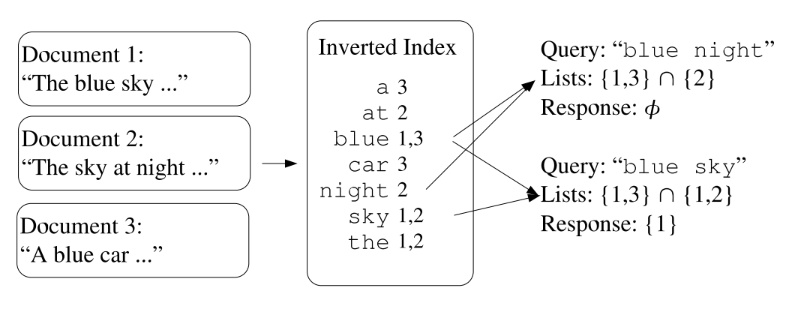
\includegraphics[width=10cm]{images/inverted_index.png}
     \caption{
An illustration of an inverted index featuring three documents. All tokens are included in this example, and the sole text normalization applied is converting all tokens to lowercase. Queries that involve multiple keywords are resolved using set operations. [3]}
     \label{fig:google-arch}
\end{figure}

Given that the inverted list can be implemented as a hashmap or dictionary in Python, where the average time complexity of a hashmap operation is O(1), the process of finding all the documents containing the query |q| has an overall time complexity of O(|q| * 1), which simplifies to O(|q|). The next step involves merging the resulting documents for each term in the query q. The time complexity of merging two sorted lists is O(n + m), where "n" is the length of the first list, and "m" is the length of the second list. Since there will be a resulting list for each term in the query q, the number of lists to merge is |q|. Consequently, the time complexity of the inverted list becomes 𝑂( |𝑞| ∗ |𝐿|), where |𝐿| represents the average length of the posting list.

It is worth noting that both |q| and |L| are typically small. The essential advantage of using the inverted list is that it makes indexing independent of the document length |D|, significantly improving performance.

\section{Ranking}
\label{sec:ranking}
As discussed, the indexing process prepares a hashmap that can be looked up to find relevant terms that match the search query; however, one needs to rank the returned result based on relevance. For example, a user searching for "what is Freiburg?" will be expecting a result about Freiburg and not to return all documents that contain tokens like "what" and "is", which are less important than the most informative term in the sentence which is "Freiburg". There are many algorithms for document ranking. However, in this thesis, BM25 will be adopted. 

\begin{equation}
BM25\_score = tf^*.\log_2(\frac{N}{df})
\label{eq:depth}
\end{equation}
\begin{equation}
tf^* = \frac{tf.(k+1)}{k.\alpha+tf}
\label{eq:depth}
\end{equation}
\begin{equation}
\alpha = \frac{1-b+b.DL}{AVDL}
\label{eq:depth}
\end{equation}

\textit{N} = Total number of docuemnts, \textit{tf} = term frequency, the number of times a word occurs in a document, \textit{df} = docuemnt frequency, The number of documents containing a particular word, \textit{DL} = document length, \textit{AVDL} =
average document length (measured in number of words).

Parameter b prevents the impact of document length normalization. It is a numeric value within the range of 0 to 1. When "b" is set to 0, there is no normalization, implying that longer documents do not face any penalties. In contrast, a value of 1 indicates complete normalization, where longer documents are penalized in proportion to their length. The default value will be set in the implementation is 0.75.

The parameter "k" governs the impact of term frequency saturation in scoring. It is a positive parameter that dictates the speed at which the term frequency component of the score achieves its peak value. When "k1" is set to 0, there is no consideration of term frequency, implying that the score remains unaffected by the number of times query terms appear in the document. On the other hand, when "k" is set to a significant value, more weight is given to term frequency, and the score escalates linearly with term frequency. The default value will be set in the implementation is 1.75.

The following example dives into the details of the BM25 equation and how it impacts ranking. Table \ref{table:bm25-documents} shows a list of documents as an example of an input to be indexed and ranked against different search queries. We start by calculating the variables needed to find the BM25 scores for each term in a document.    

Given that we have three documents, we set the variable "N" to 3. In the next step, we calculate each document's length (DF), resulting in {1: 26, 2: 21, 3: 49}. The average document length (AVDL) is determined to be 32. Substituting these values into the equation, we obtain the inverted list shown in Table \ref{table:bm25-result}.

\begin{table}[ht] 
{\footnotesize
\begin{tabular}{ P{2.5cm} ||P{11.1cm}  }      % centered columns (3 columns) 
 \hline \hline
Document ID & Document content\T\B 
\\ 
\hline
1 & The University of Freiburg, officially the Albert Ludwig University of Freiburg, is a public research university located in Freiburg im Breisgau, Baden-Württemberg, Germany.\T\B 
\\ 
\hline
2 & Freiburg im Breisgau, usually called simply Freiburg, is an independent city in the state of Baden-Württemberg in Germany.\T\B 
\\ 
\hline
3 & A university from Latin universitas 'a whole' is an institution of higher (or tertiary) education and research which awards academic degrees in several academic disciplines. Universities typically offer both undergraduate and postgraduate programs. In the United States, the designation is reserved for colleges that have a graduate school.\T\B 
\\ 
\hline \hline
    \end{tabular}
}
  \captionsetup{justification=centering,margin=2cm}
  \caption{Documents content used as an example of MB25 ranking.}
  \label{table:bm25-documents}
\end{table}

When we analyze the data in Table \ref{table:bm25-result}, it becomes evident that tokens shared by all three documents, such as 'the,' 'of,' and 'is,' have corresponding scores of 0. When dealing with common search terms, assigning lower importance or weight to the search query is advisable. For instance, users frequently search for queries like 'What is ...,' 'who is ...,' and 'Where is ...,' which include common but less informative words like 'What,' 'Who,' 'Where,' and 'is.' In such cases, the terms following these common words should be given greater value and weight.

On the other hand, unique words like 'albert' and 'ludwig' receive high scores since they are exclusive to a single document. Words such as 'freiburg' and 'university' have varying scores for each document, depending on their relative occurrences in relation to the document's length.

\begin{table}[ht] 
{\footnotesize
\begin{tabular}{ P{2.5cm} ||P{11.1cm}  }      % centered columns (3 columns) 
 \hline \hline
\textbf{Token} & \textbf{(Doc. ID, BM25 Score)}\T\B 
\\ 
\hline
the & (1, 0.0), (2, 0.0), (3, 0.0) \T\B 
\\ 
\hline
university &  (1, 1.071), (3, 0.466) \T\B 
\\ 
\hline
of  &  (1, 0.0), (2, 0.0), (3, 0.0) \T\B 
\\
\hline
freiburg  &  (1, 1.071), (2, 0.975) \T\B 
\\ 
\hline
officially  &  (1, 1.740) \T\B 
\\ 
\hline
albert  & (1, 1.740)\T\B 
\\ 
\hline
ludwig  &  (1, 1.740) \T\B 
\\ 
\hline
is  & (1, 0.0), (2, 0.0), (3, 0.0) \T\B 
\\ 
\hline
a  & (1, 0.642), (3, 0.885) \T\B 
\\ 
\hline
public  &  (1, 1.740) \T\B 
\\ 
\hline \hline
    \end{tabular}
}
  \captionsetup{justification=centering,margin=2cm}
  \caption{The first ten tokens from the resulting inverted index and the corresponding document scores. }
  \label{table:bm25-result}
\end{table}

A user's query for 'university of Freiburg' will yield the following results: (1, 2.142), (2, 0.975), (3, 0.466). The initial document with ID 1 receives the highest score since it encompasses both of the query terms. This outcome aligns with expectations, given that the first document is indeed about the University of Freiburg.

However, the concern regarding relevancy lies in the two primary keywords, "university" and "Freiburg," mentioned in documents 2 and 3. The question then becomes, which one should be prioritized in this scenario? This distinction can be influenced by adjusting the values of the "b" and "k" parameters. In this case, document 2 takes importance over document 3 because the term "Freiburg" is repeated twice, and the document itself is shorter than document 3.

The subsequent section will delve into how one can further refine the document ranking process.


\section{Fuzzy Search}
Frequently, users make spelling errors in their input queries or may employ American English spellings, such as "color," which are equivalent to British English spellings, like "colour." It would be less than ideal to return no results solely because the user chose a word variant over another. Other situations may occur where users need clarification about the correct spelling of a new term or someone's name.

Fuzzy search is a technique used in natural language processing (NLP) and information retrieval to find approximate matches for a given query or search term, even when the exact spelling or wording might not be present in the target text. This is particularly useful when dealing with typos, misspellings, phrasing variations, or other minor deviations from the original text.

Fuzzy search algorithms typically involve techniques like Levenshtein distance (edit distance), which calculates the minimum number of single-character edits (insertions, deletions, substitutions) required to change one string into another. Other techniques include using phonetic algorithms to find similar-sounding words or tokenization and comparing word n-grams to identify overlapping substrings. The greater the shared substring between the two texts, the more likely this is the intended word the user was trying to search for.


Considering two character strings, s1 and s2, the edit distance that separates them represents the minimal count of edit operations needed to transform s1 into s2. The typical edit operations permitted for this purpose include inserting a character into a string, deleting a character from a string, and replacing a character within a string with another character. In the context of these operations, the term "Levenshtein distance" is sometimes used interchangeably with edit distance. For example, the edit distance between "black" and "back" is one.


Q-grams can be used to implement the edit distance. For a string x, and an integer q ∈ N, the multiset of q-grams, denoted by Q q(x), , consists of all substrings of length q 3("freiburg") = { "fre", "rei", "eib", "ibu", "bur", "urg" }
We define it as a multiset because the same q-gram may occur multiple times and we want to know when it does 

Q 3("ababa") = { "aba", "bab", "aba" }

The number of q-grams of a string x is:

|Q q(x)| = |x| - q + 1

Similar words have many q-grams in common, that's why it can be used to find similar words. 
Lemma: for strings x and y: |Q q(x) \ Q q(y)| ≤ q ∙ ED(x, y)
Understand: A \ B denotes the set difference, that is, the elements of A without the elements from B If B is very similar to A, then A \ B is small [13]
Example:
x = freiburgerin, y = breifurgerin, ED(x, y) = Q 2(x) = { fr, re, ei, ib, bu, ur, rg, ge, er, ri, in } Q 2(y) = { br, re, ei, if, fu, ur, rg, ge, er, ri, in } 
Q 2(x) \ Q 2(y) = {fr, ib, bu}
|Q 2(x) \ Q 2(y)| = 3

To implement fuzzy search with q-gram, one can use Q-gram index. For each q-gram of a string from D, store an inverted list of all strings from D containing it, sorted lexicographically

\$fr : frankfurt, freiburg, freetown, fresno, …

More information about the implementation will be discussed in the approach section.
